% Created by tikzDevice version 0.12.6 on 2025-02-15 03:33:33
% !TEX encoding = UTF-8 Unicode
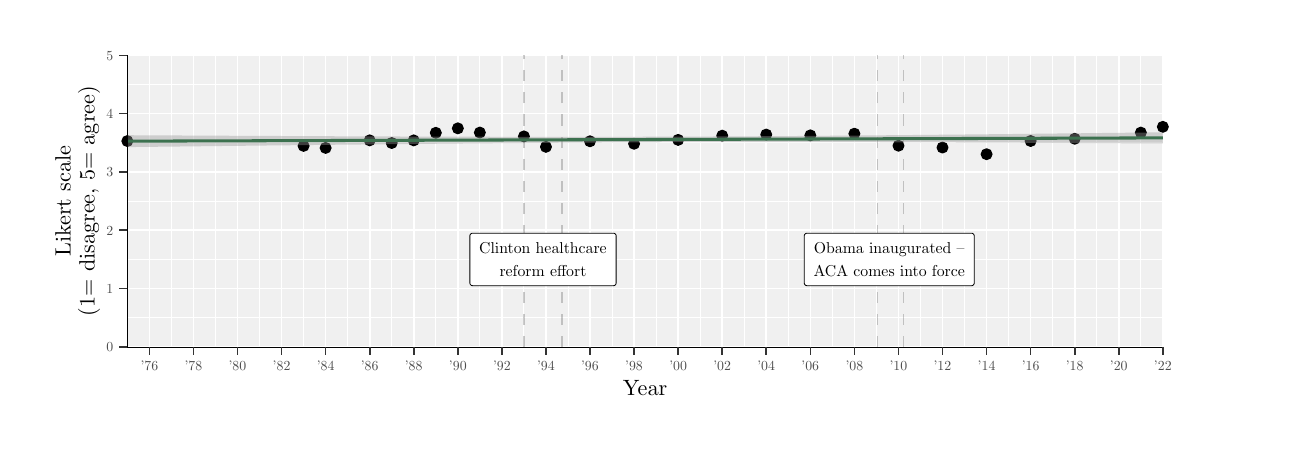
\begin{tikzpicture}[x=1pt,y=1pt]
\definecolor{fillColor}{RGB}{255,255,255}
\path[use as bounding box,fill=fillColor,fill opacity=0.00] (0,0) rectangle (455.30,144.54);
\begin{scope}
\path[clip] (  0.00,  0.00) rectangle (455.30,144.54);
\definecolor{drawColor}{RGB}{255,255,255}
\definecolor{fillColor}{RGB}{255,255,255}

\path[draw=drawColor,line width= 0.6pt,line join=round,line cap=round,fill=fillColor] ( -0.00,  0.00) rectangle (455.30,144.54);
\end{scope}
\begin{scope}
\path[clip] (  0.00,  0.00) rectangle (455.30,144.54);
\definecolor{fillColor}{gray}{0.94}

\path[fill=fillColor] ( 35.90, 29.18) rectangle (410.30,134.54);
\definecolor{drawColor}{RGB}{255,255,255}

\path[draw=drawColor,line width= 0.3pt,line join=round] ( 35.90, 39.72) --
	(410.30, 39.72);

\path[draw=drawColor,line width= 0.3pt,line join=round] ( 35.90, 60.79) --
	(410.30, 60.79);

\path[draw=drawColor,line width= 0.3pt,line join=round] ( 35.90, 81.86) --
	(410.30, 81.86);

\path[draw=drawColor,line width= 0.3pt,line join=round] ( 35.90,102.93) --
	(410.30,102.93);

\path[draw=drawColor,line width= 0.3pt,line join=round] ( 35.90,124.00) --
	(410.30,124.00);

\path[draw=drawColor,line width= 0.3pt,line join=round] ( 36.01, 29.18) --
	( 36.01,134.54);

\path[draw=drawColor,line width= 0.3pt,line join=round] ( 51.94, 29.18) --
	( 51.94,134.54);

\path[draw=drawColor,line width= 0.3pt,line join=round] ( 67.86, 29.18) --
	( 67.86,134.54);

\path[draw=drawColor,line width= 0.3pt,line join=round] ( 83.78, 29.18) --
	( 83.78,134.54);

\path[draw=drawColor,line width= 0.3pt,line join=round] ( 99.70, 29.18) --
	( 99.70,134.54);

\path[draw=drawColor,line width= 0.3pt,line join=round] (115.62, 29.18) --
	(115.62,134.54);

\path[draw=drawColor,line width= 0.3pt,line join=round] (131.55, 29.18) --
	(131.55,134.54);

\path[draw=drawColor,line width= 0.3pt,line join=round] (147.47, 29.18) --
	(147.47,134.54);

\path[draw=drawColor,line width= 0.3pt,line join=round] (163.39, 29.18) --
	(163.39,134.54);

\path[draw=drawColor,line width= 0.3pt,line join=round] (179.31, 29.18) --
	(179.31,134.54);

\path[draw=drawColor,line width= 0.3pt,line join=round] (195.24, 29.18) --
	(195.24,134.54);

\path[draw=drawColor,line width= 0.3pt,line join=round] (211.16, 29.18) --
	(211.16,134.54);

\path[draw=drawColor,line width= 0.3pt,line join=round] (227.08, 29.18) --
	(227.08,134.54);

\path[draw=drawColor,line width= 0.3pt,line join=round] (243.00, 29.18) --
	(243.00,134.54);

\path[draw=drawColor,line width= 0.3pt,line join=round] (258.93, 29.18) --
	(258.93,134.54);

\path[draw=drawColor,line width= 0.3pt,line join=round] (274.85, 29.18) --
	(274.85,134.54);

\path[draw=drawColor,line width= 0.3pt,line join=round] (290.77, 29.18) --
	(290.77,134.54);

\path[draw=drawColor,line width= 0.3pt,line join=round] (306.69, 29.18) --
	(306.69,134.54);

\path[draw=drawColor,line width= 0.3pt,line join=round] (322.61, 29.18) --
	(322.61,134.54);

\path[draw=drawColor,line width= 0.3pt,line join=round] (338.54, 29.18) --
	(338.54,134.54);

\path[draw=drawColor,line width= 0.3pt,line join=round] (354.46, 29.18) --
	(354.46,134.54);

\path[draw=drawColor,line width= 0.3pt,line join=round] (370.38, 29.18) --
	(370.38,134.54);

\path[draw=drawColor,line width= 0.3pt,line join=round] (386.30, 29.18) --
	(386.30,134.54);

\path[draw=drawColor,line width= 0.3pt,line join=round] (402.23, 29.18) --
	(402.23,134.54);

\path[draw=drawColor,line width= 0.6pt,line join=round] ( 35.90, 29.18) --
	(410.30, 29.18);

\path[draw=drawColor,line width= 0.6pt,line join=round] ( 35.90, 50.25) --
	(410.30, 50.25);

\path[draw=drawColor,line width= 0.6pt,line join=round] ( 35.90, 71.32) --
	(410.30, 71.32);

\path[draw=drawColor,line width= 0.6pt,line join=round] ( 35.90, 92.40) --
	(410.30, 92.40);

\path[draw=drawColor,line width= 0.6pt,line join=round] ( 35.90,113.47) --
	(410.30,113.47);

\path[draw=drawColor,line width= 0.6pt,line join=round] ( 35.90,134.54) --
	(410.30,134.54);

\path[draw=drawColor,line width= 0.6pt,line join=round] ( 43.97, 29.18) --
	( 43.97,134.54);

\path[draw=drawColor,line width= 0.6pt,line join=round] ( 59.90, 29.18) --
	( 59.90,134.54);

\path[draw=drawColor,line width= 0.6pt,line join=round] ( 75.81, 29.18) --
	( 75.81,134.54);

\path[draw=drawColor,line width= 0.6pt,line join=round] ( 91.75, 29.18) --
	( 91.75,134.54);

\path[draw=drawColor,line width= 0.6pt,line join=round] (107.66, 29.18) --
	(107.66,134.54);

\path[draw=drawColor,line width= 0.6pt,line join=round] (123.59, 29.18) --
	(123.59,134.54);

\path[draw=drawColor,line width= 0.6pt,line join=round] (139.50, 29.18) --
	(139.50,134.54);

\path[draw=drawColor,line width= 0.6pt,line join=round] (155.44, 29.18) --
	(155.44,134.54);

\path[draw=drawColor,line width= 0.6pt,line join=round] (171.35, 29.18) --
	(171.35,134.54);

\path[draw=drawColor,line width= 0.6pt,line join=round] (187.28, 29.18) --
	(187.28,134.54);

\path[draw=drawColor,line width= 0.6pt,line join=round] (203.19, 29.18) --
	(203.19,134.54);

\path[draw=drawColor,line width= 0.6pt,line join=round] (219.12, 29.18) --
	(219.12,134.54);

\path[draw=drawColor,line width= 0.6pt,line join=round] (235.04, 29.18) --
	(235.04,134.54);

\path[draw=drawColor,line width= 0.6pt,line join=round] (250.97, 29.18) --
	(250.97,134.54);

\path[draw=drawColor,line width= 0.6pt,line join=round] (266.88, 29.18) --
	(266.88,134.54);

\path[draw=drawColor,line width= 0.6pt,line join=round] (282.81, 29.18) --
	(282.81,134.54);

\path[draw=drawColor,line width= 0.6pt,line join=round] (298.73, 29.18) --
	(298.73,134.54);

\path[draw=drawColor,line width= 0.6pt,line join=round] (314.66, 29.18) --
	(314.66,134.54);

\path[draw=drawColor,line width= 0.6pt,line join=round] (330.57, 29.18) --
	(330.57,134.54);

\path[draw=drawColor,line width= 0.6pt,line join=round] (346.50, 29.18) --
	(346.50,134.54);

\path[draw=drawColor,line width= 0.6pt,line join=round] (362.41, 29.18) --
	(362.41,134.54);

\path[draw=drawColor,line width= 0.6pt,line join=round] (378.35, 29.18) --
	(378.35,134.54);

\path[draw=drawColor,line width= 0.6pt,line join=round] (394.26, 29.18) --
	(394.26,134.54);

\path[draw=drawColor,line width= 0.6pt,line join=round] (410.19, 29.18) --
	(410.19,134.54);
\definecolor{drawColor}{RGB}{0,0,0}

\path[draw=drawColor,draw opacity=0.20,line width= 0.6pt,dash pattern=on 4pt off 4pt ,line join=round] (179.32, 29.18) -- (179.32,134.54);

\path[draw=drawColor,draw opacity=0.20,line width= 0.6pt,dash pattern=on 4pt off 4pt ,line join=round] (193.12, 29.18) -- (193.12,134.54);

\path[draw=drawColor,draw opacity=0.20,line width= 0.6pt,dash pattern=on 4pt off 4pt ,line join=round] (307.12, 29.18) -- (307.12,134.54);

\path[draw=drawColor,draw opacity=0.20,line width= 0.6pt,dash pattern=on 4pt off 4pt ,line join=round] (316.42, 29.18) -- (316.42,134.54);
\definecolor{drawColor}{RGB}{0,0,0}
\definecolor{fillColor}{RGB}{0,0,0}

\path[draw=drawColor,line width= 0.4pt,line join=round,line cap=round,fill=fillColor] ( 36.01,103.57) circle (  1.96);

\path[draw=drawColor,line width= 0.4pt,line join=round,line cap=round,fill=fillColor] ( 99.70,101.82) circle (  1.96);

\path[draw=drawColor,line width= 0.4pt,line join=round,line cap=round,fill=fillColor] (107.66,101.09) circle (  1.96);

\path[draw=drawColor,line width= 0.4pt,line join=round,line cap=round,fill=fillColor] (123.59,103.82) circle (  1.96);

\path[draw=drawColor,line width= 0.4pt,line join=round,line cap=round,fill=fillColor] (131.55,102.86) circle (  1.96);

\path[draw=drawColor,line width= 0.4pt,line join=round,line cap=round,fill=fillColor] (139.50,103.81) circle (  1.96);

\path[draw=drawColor,line width= 0.4pt,line join=round,line cap=round,fill=fillColor] (147.48,106.55) circle (  1.96);

\path[draw=drawColor,line width= 0.4pt,line join=round,line cap=round,fill=fillColor] (155.44,108.16) circle (  1.96);

\path[draw=drawColor,line width= 0.4pt,line join=round,line cap=round,fill=fillColor] (163.39,106.64) circle (  1.96);

\path[draw=drawColor,line width= 0.4pt,line join=round,line cap=round,fill=fillColor] (179.32,105.25) circle (  1.96);

\path[draw=drawColor,line width= 0.4pt,line join=round,line cap=round,fill=fillColor] (187.28,101.48) circle (  1.96);

\path[draw=drawColor,line width= 0.4pt,line join=round,line cap=round,fill=fillColor] (203.19,103.48) circle (  1.96);

\path[draw=drawColor,line width= 0.4pt,line join=round,line cap=round,fill=fillColor] (219.12,102.59) circle (  1.96);

\path[draw=drawColor,line width= 0.4pt,line join=round,line cap=round,fill=fillColor] (235.04,103.99) circle (  1.96);

\path[draw=drawColor,line width= 0.4pt,line join=round,line cap=round,fill=fillColor] (250.97,105.51) circle (  1.96);

\path[draw=drawColor,line width= 0.4pt,line join=round,line cap=round,fill=fillColor] (266.88,105.91) circle (  1.96);

\path[draw=drawColor,line width= 0.4pt,line join=round,line cap=round,fill=fillColor] (282.81,105.62) circle (  1.96);

\path[draw=drawColor,line width= 0.4pt,line join=round,line cap=round,fill=fillColor] (298.73,106.23) circle (  1.96);

\path[draw=drawColor,line width= 0.4pt,line join=round,line cap=round,fill=fillColor] (314.66,101.89) circle (  1.96);

\path[draw=drawColor,line width= 0.4pt,line join=round,line cap=round,fill=fillColor] (330.57,101.23) circle (  1.96);

\path[draw=drawColor,line width= 0.4pt,line join=round,line cap=round,fill=fillColor] (346.50, 98.82) circle (  1.96);

\path[draw=drawColor,line width= 0.4pt,line join=round,line cap=round,fill=fillColor] (362.41,103.59) circle (  1.96);

\path[draw=drawColor,line width= 0.4pt,line join=round,line cap=round,fill=fillColor] (378.35,104.40) circle (  1.96);

\path[draw=drawColor,line width= 0.4pt,line join=round,line cap=round,fill=fillColor] (402.24,106.62) circle (  1.96);

\path[draw=drawColor,line width= 0.4pt,line join=round,line cap=round,fill=fillColor] (410.19,108.71) circle (  1.96);
\definecolor{fillColor}{RGB}{153,153,153}

\path[fill=fillColor,fill opacity=0.40] ( 36.01,105.68) --
	( 40.75,105.65) --
	( 45.49,105.63) --
	( 50.22,105.60) --
	( 54.96,105.58) --
	( 59.70,105.55) --
	( 64.43,105.53) --
	( 69.17,105.50) --
	( 73.90,105.48) --
	( 78.64,105.45) --
	( 83.38,105.43) --
	( 88.11,105.41) --
	( 92.85,105.39) --
	( 97.59,105.36) --
	(102.32,105.34) --
	(107.06,105.32) --
	(111.80,105.30) --
	(116.53,105.28) --
	(121.27,105.26) --
	(126.01,105.24) --
	(130.74,105.23) --
	(135.48,105.21) --
	(140.21,105.19) --
	(144.95,105.18) --
	(149.69,105.16) --
	(154.42,105.15) --
	(159.16,105.14) --
	(163.90,105.13) --
	(168.63,105.12) --
	(173.37,105.11) --
	(178.11,105.10) --
	(182.84,105.10) --
	(187.58,105.09) --
	(192.32,105.09) --
	(197.05,105.09) --
	(201.79,105.09) --
	(206.53,105.10) --
	(211.26,105.10) --
	(216.00,105.11) --
	(220.73,105.12) --
	(225.47,105.13) --
	(230.21,105.14) --
	(234.94,105.16) --
	(239.68,105.18) --
	(244.42,105.20) --
	(249.15,105.22) --
	(253.89,105.24) --
	(258.63,105.27) --
	(263.36,105.30) --
	(268.10,105.33) --
	(272.84,105.36) --
	(277.57,105.39) --
	(282.31,105.43) --
	(287.04,105.46) --
	(291.78,105.50) --
	(296.52,105.54) --
	(301.25,105.58) --
	(305.99,105.62) --
	(310.73,105.67) --
	(315.46,105.71) --
	(320.20,105.76) --
	(324.94,105.80) --
	(329.67,105.85) --
	(334.41,105.90) --
	(339.15,105.94) --
	(343.88,105.99) --
	(348.62,106.04) --
	(353.35,106.09) --
	(358.09,106.14) --
	(362.83,106.19) --
	(367.56,106.25) --
	(372.30,106.30) --
	(377.04,106.35) --
	(381.77,106.40) --
	(386.51,106.46) --
	(391.25,106.51) --
	(395.98,106.56) --
	(400.72,106.62) --
	(405.46,106.67) --
	(410.19,106.73) --
	(410.19,102.70) --
	(405.46,102.72) --
	(400.72,102.75) --
	(395.98,102.77) --
	(391.25,102.80) --
	(386.51,102.82) --
	(381.77,102.84) --
	(377.04,102.87) --
	(372.30,102.89) --
	(367.56,102.91) --
	(362.83,102.93) --
	(358.09,102.96) --
	(353.35,102.98) --
	(348.62,103.00) --
	(343.88,103.02) --
	(339.15,103.03) --
	(334.41,103.05) --
	(329.67,103.07) --
	(324.94,103.09) --
	(320.20,103.10) --
	(315.46,103.12) --
	(310.73,103.13) --
	(305.99,103.14) --
	(301.25,103.16) --
	(296.52,103.17) --
	(291.78,103.18) --
	(287.04,103.18) --
	(282.31,103.19) --
	(277.57,103.19) --
	(272.84,103.20) --
	(268.10,103.20) --
	(263.36,103.20) --
	(258.63,103.20) --
	(253.89,103.19) --
	(249.15,103.19) --
	(244.42,103.18) --
	(239.68,103.17) --
	(234.94,103.16) --
	(230.21,103.14) --
	(225.47,103.13) --
	(220.73,103.11) --
	(216.00,103.09) --
	(211.26,103.07) --
	(206.53,103.04) --
	(201.79,103.01) --
	(197.05,102.99) --
	(192.32,102.96) --
	(187.58,102.92) --
	(182.84,102.89) --
	(178.11,102.85) --
	(173.37,102.82) --
	(168.63,102.78) --
	(163.90,102.74) --
	(159.16,102.70) --
	(154.42,102.66) --
	(149.69,102.61) --
	(144.95,102.57) --
	(140.21,102.52) --
	(135.48,102.48) --
	(130.74,102.43) --
	(126.01,102.38) --
	(121.27,102.33) --
	(116.53,102.29) --
	(111.80,102.24) --
	(107.06,102.19) --
	(102.32,102.13) --
	( 97.59,102.08) --
	( 92.85,102.03) --
	( 88.11,101.98) --
	( 83.38,101.93) --
	( 78.64,101.87) --
	( 73.90,101.82) --
	( 69.17,101.77) --
	( 64.43,101.71) --
	( 59.70,101.66) --
	( 54.96,101.60) --
	( 50.22,101.55) --
	( 45.49,101.49) --
	( 40.75,101.44) --
	( 36.01,101.38) --
	cycle;

\path[] ( 36.01,105.68) --
	( 40.75,105.65) --
	( 45.49,105.63) --
	( 50.22,105.60) --
	( 54.96,105.58) --
	( 59.70,105.55) --
	( 64.43,105.53) --
	( 69.17,105.50) --
	( 73.90,105.48) --
	( 78.64,105.45) --
	( 83.38,105.43) --
	( 88.11,105.41) --
	( 92.85,105.39) --
	( 97.59,105.36) --
	(102.32,105.34) --
	(107.06,105.32) --
	(111.80,105.30) --
	(116.53,105.28) --
	(121.27,105.26) --
	(126.01,105.24) --
	(130.74,105.23) --
	(135.48,105.21) --
	(140.21,105.19) --
	(144.95,105.18) --
	(149.69,105.16) --
	(154.42,105.15) --
	(159.16,105.14) --
	(163.90,105.13) --
	(168.63,105.12) --
	(173.37,105.11) --
	(178.11,105.10) --
	(182.84,105.10) --
	(187.58,105.09) --
	(192.32,105.09) --
	(197.05,105.09) --
	(201.79,105.09) --
	(206.53,105.10) --
	(211.26,105.10) --
	(216.00,105.11) --
	(220.73,105.12) --
	(225.47,105.13) --
	(230.21,105.14) --
	(234.94,105.16) --
	(239.68,105.18) --
	(244.42,105.20) --
	(249.15,105.22) --
	(253.89,105.24) --
	(258.63,105.27) --
	(263.36,105.30) --
	(268.10,105.33) --
	(272.84,105.36) --
	(277.57,105.39) --
	(282.31,105.43) --
	(287.04,105.46) --
	(291.78,105.50) --
	(296.52,105.54) --
	(301.25,105.58) --
	(305.99,105.62) --
	(310.73,105.67) --
	(315.46,105.71) --
	(320.20,105.76) --
	(324.94,105.80) --
	(329.67,105.85) --
	(334.41,105.90) --
	(339.15,105.94) --
	(343.88,105.99) --
	(348.62,106.04) --
	(353.35,106.09) --
	(358.09,106.14) --
	(362.83,106.19) --
	(367.56,106.25) --
	(372.30,106.30) --
	(377.04,106.35) --
	(381.77,106.40) --
	(386.51,106.46) --
	(391.25,106.51) --
	(395.98,106.56) --
	(400.72,106.62) --
	(405.46,106.67) --
	(410.19,106.73);

\path[] (410.19,102.70) --
	(405.46,102.72) --
	(400.72,102.75) --
	(395.98,102.77) --
	(391.25,102.80) --
	(386.51,102.82) --
	(381.77,102.84) --
	(377.04,102.87) --
	(372.30,102.89) --
	(367.56,102.91) --
	(362.83,102.93) --
	(358.09,102.96) --
	(353.35,102.98) --
	(348.62,103.00) --
	(343.88,103.02) --
	(339.15,103.03) --
	(334.41,103.05) --
	(329.67,103.07) --
	(324.94,103.09) --
	(320.20,103.10) --
	(315.46,103.12) --
	(310.73,103.13) --
	(305.99,103.14) --
	(301.25,103.16) --
	(296.52,103.17) --
	(291.78,103.18) --
	(287.04,103.18) --
	(282.31,103.19) --
	(277.57,103.19) --
	(272.84,103.20) --
	(268.10,103.20) --
	(263.36,103.20) --
	(258.63,103.20) --
	(253.89,103.19) --
	(249.15,103.19) --
	(244.42,103.18) --
	(239.68,103.17) --
	(234.94,103.16) --
	(230.21,103.14) --
	(225.47,103.13) --
	(220.73,103.11) --
	(216.00,103.09) --
	(211.26,103.07) --
	(206.53,103.04) --
	(201.79,103.01) --
	(197.05,102.99) --
	(192.32,102.96) --
	(187.58,102.92) --
	(182.84,102.89) --
	(178.11,102.85) --
	(173.37,102.82) --
	(168.63,102.78) --
	(163.90,102.74) --
	(159.16,102.70) --
	(154.42,102.66) --
	(149.69,102.61) --
	(144.95,102.57) --
	(140.21,102.52) --
	(135.48,102.48) --
	(130.74,102.43) --
	(126.01,102.38) --
	(121.27,102.33) --
	(116.53,102.29) --
	(111.80,102.24) --
	(107.06,102.19) --
	(102.32,102.13) --
	( 97.59,102.08) --
	( 92.85,102.03) --
	( 88.11,101.98) --
	( 83.38,101.93) --
	( 78.64,101.87) --
	( 73.90,101.82) --
	( 69.17,101.77) --
	( 64.43,101.71) --
	( 59.70,101.66) --
	( 54.96,101.60) --
	( 50.22,101.55) --
	( 45.49,101.49) --
	( 40.75,101.44) --
	( 36.01,101.38);
\definecolor{drawColor}{RGB}{60,113,79}

\path[draw=drawColor,line width= 1.1pt,line join=round] ( 36.01,103.53) --
	( 40.75,103.54) --
	( 45.49,103.56) --
	( 50.22,103.57) --
	( 54.96,103.59) --
	( 59.70,103.60) --
	( 64.43,103.62) --
	( 69.17,103.63) --
	( 73.90,103.65) --
	( 78.64,103.66) --
	( 83.38,103.68) --
	( 88.11,103.69) --
	( 92.85,103.71) --
	( 97.59,103.72) --
	(102.32,103.74) --
	(107.06,103.75) --
	(111.80,103.77) --
	(116.53,103.78) --
	(121.27,103.80) --
	(126.01,103.81) --
	(130.74,103.83) --
	(135.48,103.84) --
	(140.21,103.86) --
	(144.95,103.87) --
	(149.69,103.89) --
	(154.42,103.90) --
	(159.16,103.92) --
	(163.90,103.93) --
	(168.63,103.95) --
	(173.37,103.96) --
	(178.11,103.98) --
	(182.84,103.99) --
	(187.58,104.01) --
	(192.32,104.02) --
	(197.05,104.04) --
	(201.79,104.05) --
	(206.53,104.07) --
	(211.26,104.08) --
	(216.00,104.10) --
	(220.73,104.11) --
	(225.47,104.13) --
	(230.21,104.14) --
	(234.94,104.16) --
	(239.68,104.17) --
	(244.42,104.19) --
	(249.15,104.20) --
	(253.89,104.22) --
	(258.63,104.23) --
	(263.36,104.25) --
	(268.10,104.26) --
	(272.84,104.28) --
	(277.57,104.29) --
	(282.31,104.31) --
	(287.04,104.32) --
	(291.78,104.34) --
	(296.52,104.35) --
	(301.25,104.37) --
	(305.99,104.38) --
	(310.73,104.40) --
	(315.46,104.41) --
	(320.20,104.43) --
	(324.94,104.44) --
	(329.67,104.46) --
	(334.41,104.47) --
	(339.15,104.49) --
	(343.88,104.50) --
	(348.62,104.52) --
	(353.35,104.53) --
	(358.09,104.55) --
	(362.83,104.56) --
	(367.56,104.58) --
	(372.30,104.59) --
	(377.04,104.61) --
	(381.77,104.62) --
	(386.51,104.64) --
	(391.25,104.65) --
	(395.98,104.67) --
	(400.72,104.68) --
	(405.46,104.70) --
	(410.19,104.71);
\definecolor{drawColor}{RGB}{0,0,0}
\definecolor{fillColor}{RGB}{255,255,255}

\path[draw=drawColor,line width= 0.3pt,line join=round,line cap=round,fill=fillColor] (160.81, 51.30) --
	(211.61, 51.30) --
	(211.57, 51.31) --
	(211.74, 51.31) --
	(211.90, 51.34) --
	(212.06, 51.40) --
	(212.20, 51.49) --
	(212.33, 51.59) --
	(212.44, 51.71) --
	(212.53, 51.85) --
	(212.59, 52.01) --
	(212.63, 52.17) --
	(212.64, 52.33) --
	(212.64, 52.33) --
	(212.64, 69.24) --
	(212.64, 69.24) --
	(212.63, 69.41) --
	(212.59, 69.57) --
	(212.53, 69.72) --
	(212.44, 69.86) --
	(212.33, 69.99) --
	(212.20, 70.09) --
	(212.06, 70.17) --
	(211.90, 70.23) --
	(211.74, 70.26) --
	(211.61, 70.27) --
	(160.81, 70.27) --
	(160.93, 70.26) --
	(160.77, 70.27) --
	(160.60, 70.25) --
	(160.45, 70.21) --
	(160.30, 70.13) --
	(160.16, 70.04) --
	(160.04, 69.93) --
	(159.94, 69.79) --
	(159.86, 69.65) --
	(159.81, 69.49) --
	(159.78, 69.33) --
	(159.78, 69.24) --
	(159.78, 52.33) --
	(159.78, 52.42) --
	(159.78, 52.25) --
	(159.81, 52.09) --
	(159.86, 51.93) --
	(159.94, 51.78) --
	(160.04, 51.65) --
	(160.16, 51.54) --
	(160.30, 51.44) --
	(160.45, 51.37) --
	(160.60, 51.33) --
	(160.77, 51.31) --
	cycle;
\end{scope}
\begin{scope}
\path[clip] (  0.00,  0.00) rectangle (455.30,144.54);
\definecolor{drawColor}{RGB}{0,0,0}

\node[text=drawColor,anchor=base,inner sep=0pt, outer sep=0pt, scale=  0.57] at (186.21, 62.93) {Clinton healthcare };

\node[text=drawColor,anchor=base,inner sep=0pt, outer sep=0pt, scale=  0.57] at (186.21, 54.73) { reform effort};
\end{scope}
\begin{scope}
\path[clip] (  0.00,  0.00) rectangle (455.30,144.54);
\definecolor{drawColor}{RGB}{0,0,0}
\definecolor{fillColor}{RGB}{255,255,255}

\path[draw=drawColor,line width= 0.3pt,line join=round,line cap=round,fill=fillColor] (281.64, 51.30) --
	(341.01, 51.30) --
	(340.97, 51.31) --
	(341.13, 51.31) --
	(341.30, 51.34) --
	(341.45, 51.40) --
	(341.59, 51.49) --
	(341.72, 51.59) --
	(341.83, 51.71) --
	(341.92, 51.85) --
	(341.98, 52.01) --
	(342.02, 52.17) --
	(342.04, 52.33) --
	(342.04, 52.33) --
	(342.04, 69.24) --
	(342.04, 69.24) --
	(342.02, 69.41) --
	(341.98, 69.57) --
	(341.92, 69.72) --
	(341.83, 69.86) --
	(341.72, 69.99) --
	(341.59, 70.09) --
	(341.45, 70.17) --
	(341.30, 70.23) --
	(341.13, 70.26) --
	(341.01, 70.27) --
	(281.64, 70.27) --
	(281.76, 70.26) --
	(281.60, 70.27) --
	(281.43, 70.25) --
	(281.27, 70.21) --
	(281.12, 70.13) --
	(280.99, 70.04) --
	(280.87, 69.93) --
	(280.77, 69.79) --
	(280.69, 69.65) --
	(280.64, 69.49) --
	(280.61, 69.33) --
	(280.61, 69.24) --
	(280.61, 52.33) --
	(280.61, 52.42) --
	(280.61, 52.25) --
	(280.64, 52.09) --
	(280.69, 51.93) --
	(280.77, 51.78) --
	(280.87, 51.65) --
	(280.99, 51.54) --
	(281.12, 51.44) --
	(281.27, 51.37) --
	(281.43, 51.33) --
	(281.60, 51.31) --
	cycle;
\end{scope}
\begin{scope}
\path[clip] (  0.00,  0.00) rectangle (455.30,144.54);
\definecolor{drawColor}{RGB}{0,0,0}

\node[text=drawColor,anchor=base,inner sep=0pt, outer sep=0pt, scale=  0.57] at (311.32, 62.93) {Obama inaugurated -- };

\node[text=drawColor,anchor=base,inner sep=0pt, outer sep=0pt, scale=  0.57] at (311.32, 54.73) { ACA comes into force};
\end{scope}
\begin{scope}
\path[clip] (  0.00,  0.00) rectangle (455.30,144.54);
\definecolor{drawColor}{RGB}{0,0,0}

\path[draw=drawColor,line width= 0.2pt,line join=round] ( 35.90, 29.18) --
	( 35.90,134.54);
\end{scope}
\begin{scope}
\path[clip] (  0.00,  0.00) rectangle (455.30,144.54);
\definecolor{drawColor}{gray}{0.30}

\node[text=drawColor,anchor=base east,inner sep=0pt, outer sep=0pt, scale=  0.50] at ( 30.95, 27.46) {0};

\node[text=drawColor,anchor=base east,inner sep=0pt, outer sep=0pt, scale=  0.50] at ( 30.95, 48.53) {1};

\node[text=drawColor,anchor=base east,inner sep=0pt, outer sep=0pt, scale=  0.50] at ( 30.95, 69.60) {2};

\node[text=drawColor,anchor=base east,inner sep=0pt, outer sep=0pt, scale=  0.50] at ( 30.95, 90.67) {3};

\node[text=drawColor,anchor=base east,inner sep=0pt, outer sep=0pt, scale=  0.50] at ( 30.95,111.75) {4};

\node[text=drawColor,anchor=base east,inner sep=0pt, outer sep=0pt, scale=  0.50] at ( 30.95,132.82) {5};
\end{scope}
\begin{scope}
\path[clip] (  0.00,  0.00) rectangle (455.30,144.54);
\definecolor{drawColor}{gray}{0.20}

\path[draw=drawColor,line width= 0.6pt,line join=round] ( 33.15, 29.18) --
	( 35.90, 29.18);

\path[draw=drawColor,line width= 0.6pt,line join=round] ( 33.15, 50.25) --
	( 35.90, 50.25);

\path[draw=drawColor,line width= 0.6pt,line join=round] ( 33.15, 71.32) --
	( 35.90, 71.32);

\path[draw=drawColor,line width= 0.6pt,line join=round] ( 33.15, 92.40) --
	( 35.90, 92.40);

\path[draw=drawColor,line width= 0.6pt,line join=round] ( 33.15,113.47) --
	( 35.90,113.47);

\path[draw=drawColor,line width= 0.6pt,line join=round] ( 33.15,134.54) --
	( 35.90,134.54);
\end{scope}
\begin{scope}
\path[clip] (  0.00,  0.00) rectangle (455.30,144.54);
\definecolor{drawColor}{RGB}{0,0,0}

\path[draw=drawColor,line width= 0.2pt,line join=round] ( 35.90, 29.18) --
	(410.30, 29.18);
\end{scope}
\begin{scope}
\path[clip] (  0.00,  0.00) rectangle (455.30,144.54);
\definecolor{drawColor}{gray}{0.20}

\path[draw=drawColor,line width= 0.6pt,line join=round] ( 43.97, 26.43) --
	( 43.97, 29.18);

\path[draw=drawColor,line width= 0.6pt,line join=round] ( 59.90, 26.43) --
	( 59.90, 29.18);

\path[draw=drawColor,line width= 0.6pt,line join=round] ( 75.81, 26.43) --
	( 75.81, 29.18);

\path[draw=drawColor,line width= 0.6pt,line join=round] ( 91.75, 26.43) --
	( 91.75, 29.18);

\path[draw=drawColor,line width= 0.6pt,line join=round] (107.66, 26.43) --
	(107.66, 29.18);

\path[draw=drawColor,line width= 0.6pt,line join=round] (123.59, 26.43) --
	(123.59, 29.18);

\path[draw=drawColor,line width= 0.6pt,line join=round] (139.50, 26.43) --
	(139.50, 29.18);

\path[draw=drawColor,line width= 0.6pt,line join=round] (155.44, 26.43) --
	(155.44, 29.18);

\path[draw=drawColor,line width= 0.6pt,line join=round] (171.35, 26.43) --
	(171.35, 29.18);

\path[draw=drawColor,line width= 0.6pt,line join=round] (187.28, 26.43) --
	(187.28, 29.18);

\path[draw=drawColor,line width= 0.6pt,line join=round] (203.19, 26.43) --
	(203.19, 29.18);

\path[draw=drawColor,line width= 0.6pt,line join=round] (219.12, 26.43) --
	(219.12, 29.18);

\path[draw=drawColor,line width= 0.6pt,line join=round] (235.04, 26.43) --
	(235.04, 29.18);

\path[draw=drawColor,line width= 0.6pt,line join=round] (250.97, 26.43) --
	(250.97, 29.18);

\path[draw=drawColor,line width= 0.6pt,line join=round] (266.88, 26.43) --
	(266.88, 29.18);

\path[draw=drawColor,line width= 0.6pt,line join=round] (282.81, 26.43) --
	(282.81, 29.18);

\path[draw=drawColor,line width= 0.6pt,line join=round] (298.73, 26.43) --
	(298.73, 29.18);

\path[draw=drawColor,line width= 0.6pt,line join=round] (314.66, 26.43) --
	(314.66, 29.18);

\path[draw=drawColor,line width= 0.6pt,line join=round] (330.57, 26.43) --
	(330.57, 29.18);

\path[draw=drawColor,line width= 0.6pt,line join=round] (346.50, 26.43) --
	(346.50, 29.18);

\path[draw=drawColor,line width= 0.6pt,line join=round] (362.41, 26.43) --
	(362.41, 29.18);

\path[draw=drawColor,line width= 0.6pt,line join=round] (378.35, 26.43) --
	(378.35, 29.18);

\path[draw=drawColor,line width= 0.6pt,line join=round] (394.26, 26.43) --
	(394.26, 29.18);

\path[draw=drawColor,line width= 0.6pt,line join=round] (410.19, 26.43) --
	(410.19, 29.18);
\end{scope}
\begin{scope}
\path[clip] (  0.00,  0.00) rectangle (455.30,144.54);
\definecolor{drawColor}{gray}{0.30}

\node[text=drawColor,anchor=base,inner sep=0pt, outer sep=0pt, scale=  0.50] at ( 43.97, 20.79) {'76};

\node[text=drawColor,anchor=base,inner sep=0pt, outer sep=0pt, scale=  0.50] at ( 59.90, 20.79) {'78};

\node[text=drawColor,anchor=base,inner sep=0pt, outer sep=0pt, scale=  0.50] at ( 75.81, 20.79) {'80};

\node[text=drawColor,anchor=base,inner sep=0pt, outer sep=0pt, scale=  0.50] at ( 91.75, 20.79) {'82};

\node[text=drawColor,anchor=base,inner sep=0pt, outer sep=0pt, scale=  0.50] at (107.66, 20.79) {'84};

\node[text=drawColor,anchor=base,inner sep=0pt, outer sep=0pt, scale=  0.50] at (123.59, 20.79) {'86};

\node[text=drawColor,anchor=base,inner sep=0pt, outer sep=0pt, scale=  0.50] at (139.50, 20.79) {'88};

\node[text=drawColor,anchor=base,inner sep=0pt, outer sep=0pt, scale=  0.50] at (155.44, 20.79) {'90};

\node[text=drawColor,anchor=base,inner sep=0pt, outer sep=0pt, scale=  0.50] at (171.35, 20.79) {'92};

\node[text=drawColor,anchor=base,inner sep=0pt, outer sep=0pt, scale=  0.50] at (187.28, 20.79) {'94};

\node[text=drawColor,anchor=base,inner sep=0pt, outer sep=0pt, scale=  0.50] at (203.19, 20.79) {'96};

\node[text=drawColor,anchor=base,inner sep=0pt, outer sep=0pt, scale=  0.50] at (219.12, 20.79) {'98};

\node[text=drawColor,anchor=base,inner sep=0pt, outer sep=0pt, scale=  0.50] at (235.04, 20.79) {'00};

\node[text=drawColor,anchor=base,inner sep=0pt, outer sep=0pt, scale=  0.50] at (250.97, 20.79) {'02};

\node[text=drawColor,anchor=base,inner sep=0pt, outer sep=0pt, scale=  0.50] at (266.88, 20.79) {'04};

\node[text=drawColor,anchor=base,inner sep=0pt, outer sep=0pt, scale=  0.50] at (282.81, 20.79) {'06};

\node[text=drawColor,anchor=base,inner sep=0pt, outer sep=0pt, scale=  0.50] at (298.73, 20.79) {'08};

\node[text=drawColor,anchor=base,inner sep=0pt, outer sep=0pt, scale=  0.50] at (314.66, 20.79) {'10};

\node[text=drawColor,anchor=base,inner sep=0pt, outer sep=0pt, scale=  0.50] at (330.57, 20.79) {'12};

\node[text=drawColor,anchor=base,inner sep=0pt, outer sep=0pt, scale=  0.50] at (346.50, 20.79) {'14};

\node[text=drawColor,anchor=base,inner sep=0pt, outer sep=0pt, scale=  0.50] at (362.41, 20.79) {'16};

\node[text=drawColor,anchor=base,inner sep=0pt, outer sep=0pt, scale=  0.50] at (378.35, 20.79) {'18};

\node[text=drawColor,anchor=base,inner sep=0pt, outer sep=0pt, scale=  0.50] at (394.26, 20.79) {'20};

\node[text=drawColor,anchor=base,inner sep=0pt, outer sep=0pt, scale=  0.50] at (410.19, 20.79) {'22};
\end{scope}
\begin{scope}
\path[clip] (  0.00,  0.00) rectangle (455.30,144.54);
\definecolor{drawColor}{RGB}{0,0,0}

\node[text=drawColor,anchor=base,inner sep=0pt, outer sep=0pt, scale=  0.80] at (223.10, 11.56) {Year};
\end{scope}
\begin{scope}
\path[clip] (  0.00,  0.00) rectangle (455.30,144.54);
\definecolor{drawColor}{RGB}{0,0,0}

\node[text=drawColor,rotate= 90.00,anchor=base,inner sep=0pt, outer sep=0pt, scale=  0.80] at ( 15.51, 81.86) {Likert scale };

\node[text=drawColor,rotate= 90.00,anchor=base,inner sep=0pt, outer sep=0pt, scale=  0.80] at ( 24.15, 81.86) { (1= disagree, 5= agree)};
\end{scope}
\end{tikzpicture}
